\noindent
\subsection{Reviewer}
\label{reviewer}

In this section, we investigate anomalous behavior of the referees. Recall that we define the behavior of a reviewer to be anomalous if the papers accepted by her are low cited or the papers rejected by her are highly cited. As in case of the editors, here also we investigate different factors that could be indicative of such anomalous behavior.  

\subsubsection{Mean Reviewer Assignment Time (MRAT)}

%For each individual reviewer we find the time difference (in days) between two consecutive assignments. Note that we do not consider the cases where the reviewer was assigned but she declined to review it.
This is essentially same as MEAT. For a reviewer $i$, we define $MRAT_{i}$ as
\begin{center}
$MRAT_{i}=\frac{1}{n-1}\sum (\delta_{j+1} - \delta_{j})$
\end{center}
\noindent where $n$ is the total number of assignments of reviewer $i$ and $\delta_{j}$ is the date of the $j^\textrm{th}$ assignment. In figure~\ref{fig5}(a) we plot $MRAT$ (binned) and median average citation of the papers reviewed for each reviewer. We observe that papers reviewed by reviewers with low $MRAT$ (high frequency of assignment) tend to be cited less and increases as $MRAT$ increases. This is followed by again a steep decrease in citation. This indicates that the reviewers assigned very frequently are often less reliable while those assigned only occasionally are also not likely to correctly judge the quality of the paper.  

\subsubsection{Mean Report Sending Delay (MRSD)}

We argue that the time taken by a reviewer to send back the review report could be an indicator of his performance. If a reviewer on average sends back the review very quickly it is highly likely that the review was done in a hurry. Similarly, if the report was sent after being reminded by the editor numerous times, it is also highly likely the review report could be anomalous. For a reviewer we calculate the time delay between the date of her assignment and the date she sent back the report for each of her assignments. To measure $MRSD$ we calculate the mean value of all the delays. Note that we do not consider the assignments which the reviewer declined. Formally, for a reviewer $i$, we define $MRSD_{i}$ as 

\begin{center}
$MRSD_{i}=\frac{1}{n}\sum(\delta_{i}-\Delta_{i})$
\end{center}

where $n$ is the total number of assignments, $\Delta_{i}$ is the date of assignment and $\delta_{i}$ is the date when the report was received by the editor. On plotting against median average citation we observe a similar trend as was observed in case of $MRAT$ (refer to figure~\ref{fig5}(b)). Papers reviewed by reviewers with low $MRSD$ value are often less cited, indicating that reviewers sending back their report very quickly often do it in a hurry and fail to correctly judge the quality of the paper while those taking very long to send report are prone to failure as well. 

\subsubsection{Topic Diversity Index (TDI)}

JHEP associates with each submission a set of keywords which roughly indicates the domain of the work. We use these associated keywords as a proxy for topic. For each reviewer, we segregate all the keywords of the papers reviewed by her which we call the keyword corpus for the reviewer. Formally for a reviewer $i$, we define $TDI_{i}$ as 

\begin{center}
$TDI_{i}=-\sum \limits_{j} p_{j}\log p_{j}$
\end{center}

\noindent where $p_{j}$ is the proportion of keyword $j$ in the keyword corpus for reviewer $i$. We segregate the reviewers based on the diversity score and calculate the median average citation of the papers reviewed by them. We observe that the median average citation %[{\color{red}{\bf Why introduce this acronym here? Use it from the first time it has been invoked.}}] 
for reviewers with low $TDI$ are low mainly because the number of papers reviewed by them are also less. The value increases with  increasing $TDI$ (refer to figure~\ref{fig5}(c)). The reviewers with low $TDI$ are often the ones who have reviewed a very small number of papers while the reviewers with high $TDI$ are mostly assigned papers by a large number of editors. 
 
 
 
\subsubsection{Editor Diversity Index (EDI)}

Reviewers could be selected for review by a large set of editors or could only be selected by a single or a small set of editors. We check whether a reviewer selected by many editors is more reliable compared to one who is selected by a single or a very small set of editors. To this aim we assign each reviewer a score called Editor Diversity Index, $EDI_{i}$ which is defined as 

\begin{center}
$EDI_{i}=-\sum \limits_{j} p_{j}\log p_{j}$
\end{center}

where $p_{j}$ represents the proportion of times reviewer $i$ was assigned by editor $j$. We segregate the reviewers based on $EDI$ and calculate the median average citation of the papers reviewed by them. We observe that as $EDI$ increases median average citation also increases (refer to figure \ref{fig5}(d)) indicating that reviewers assigned by multiple editors are often more reliable.

\begin{table}[htpb]
\centering
\caption{Features used for detecting anomalies.}
\label{summary_stat}
\small
\begin{tabular}{|l|l|l|l|l|l|l|}
\hline
                        & Factor                                     & Mean & Median & Max & Min & \begin{tabular}[c]{@{}l@{}}St.\\ Dev\end{tabular} \\ \hline
\multirow{3}{*}{Editor} & $MEAT$         & 35.06     &  29.1      &  108.25   &  3.28   & 23.19                                                             \\  
                        & $RDI$              & 6.57     &  6.79      & 8.85    & 0.0    &  1.44                                                            \\ 
                        & $RADI$ & 8.86     & 9.21       & 11.94    & 0.0    &  1.87 
                         \\ 
                        & $SRI$ & 0.28     & 0.25       & 0.85    & 0.0    &  0.19                                                           
                        \\ \hline
\multirow{6}{*}{Reviewer} & $MRAT$       & 363.3     & 193.7       & 5389    & 26.9    & 508.9                                                             \\  
                        & $MRSD$           & 19.28     & 17.50       & 122    & 16.5    &  11.45                                                            \\  
                        & $TDI$                &  4.07    &  3.96      & 8.10    & 1.0    &  1.44                                                            \\  
                        & $EDI$               &  1.12    &   0.91     &  4.58   & 0.0    &   1.19                                                           \\  
                        & $AR$                      &  0.65    &   0.71     &   1.0  & 0.0    &    0.2                                                          \\  
                        & $MTD$                 &   3.86   &  3.12      & 69.0    & 1.0    & 4.96                                                             \\ 
                        & $DFI$                 & 0.19     & 0.12       & 1.0    & 0.0    & 0.30                                                             \\ \hline
                        
\end{tabular}
\vspace{3mm}
\end{table} 


\subsubsection{Mean Time to Decline (MTD)}

We further investigated the cases where the reviewer declined the assignment. In specific, we calculated the time delay (in days) 
between the date she was assigned and the date she conveyed her decision of declining to review. For each reviewer we define {\bf Mean Time to Delay}, $MTD_{i}$ as 

\begin{center}
$MTD_{i}= \frac{1}{d}\sum \limits_{j}(\mu_{j} - \Delta_{j})$
\end{center}

where $d$ is the number of assignments that reviewer $i$ declined and $\mu_{j}$ and $\Delta_{j}$ are respectively the date of assignments and date of reply for paper $j$ by reviewer $i$. We segregate the reviewers based on their $MTD$ values and calculate the median average citation. We observe that the reviewers who delay often in reporting their decision to the editor of being unable to review usually tend to fail in judging a paper quality when they do review (refer to figure~\ref{fig5}(f)).

\subsubsection{Acceptance Ratio (AR)}
Acceptance Ratio ($AR$) of a reviewer is defined as the proportion of papers accepted by the reviewer. For a reviewer $i$, $AR_{i}$ is formally defined as 

\begin{center}
$AR_{i}=\frac{a_{i}}{a_{i}+r_{i}}$
\end{center}

\noindent where $a_{i}$ and $r_{i}$ respectively denote the number of papers accepted and rejected by reviewer $i$. We observe that reviewers with high $AR$ often accept  less impactful papers while reviewers with very low $AR$ often fail to identify quality research (refer to figure~\ref{fig5}(e)). Note that the reviewers are segregated based on their respective $AR$ values while the median average citation is calculated. They are segregated into bins based on the $AR$ values where typically the bins are ($\geq$ 0 and $< 0.1$), ($\geq$ 0.1 and $<$ 0.2) and so on.

\begin{figure}
\centering
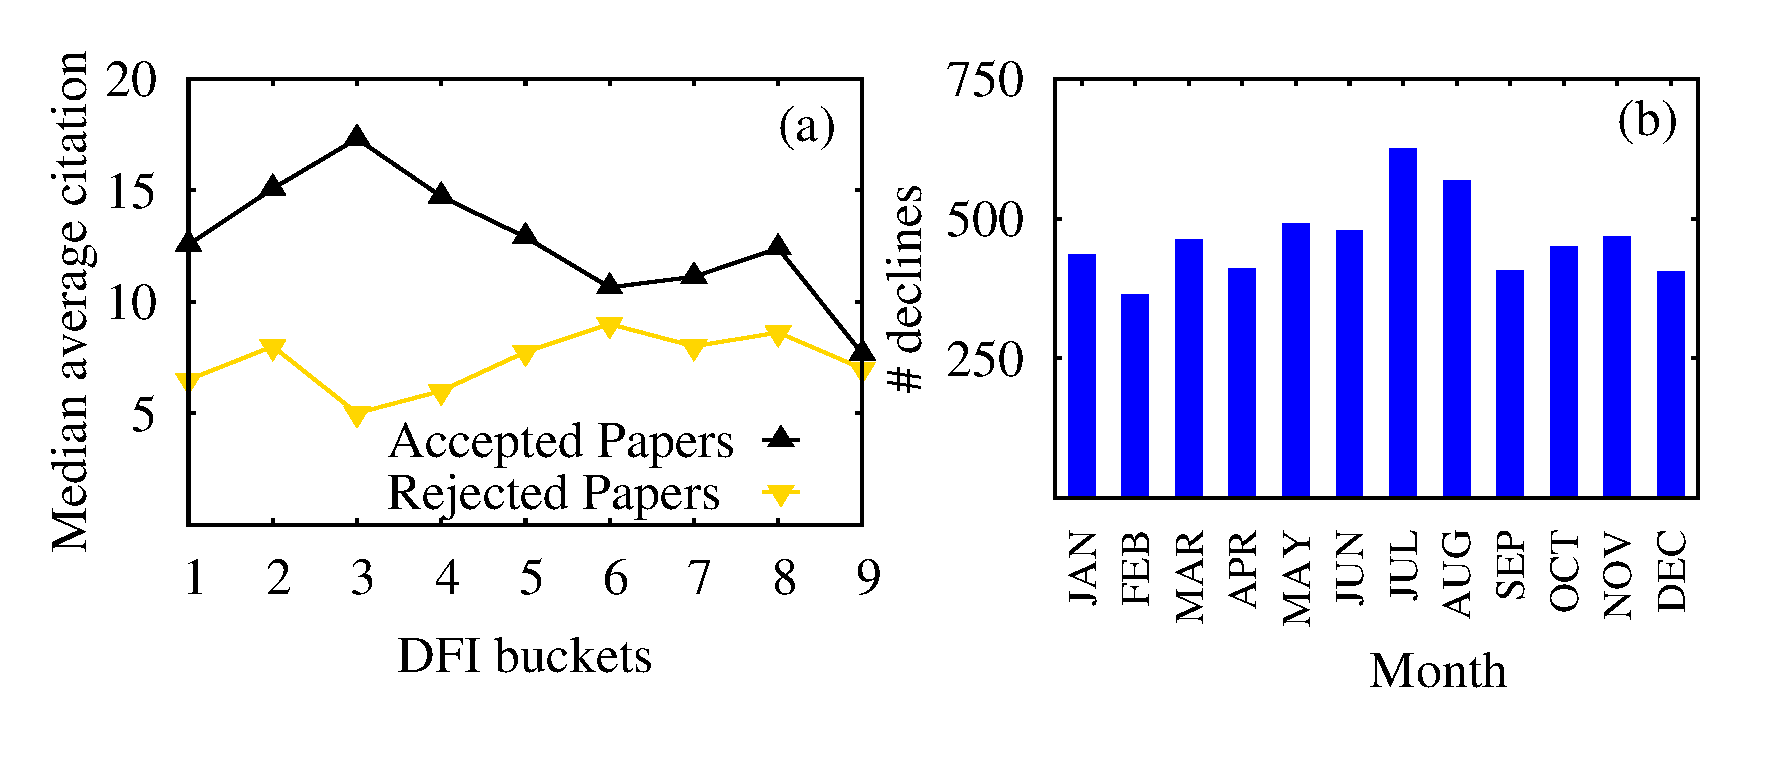
\includegraphics[scale=0.3]{./texfiles/Chapter_4/cikm/figures/DFI_dec_month.eps}
\caption{\label{fig_dfi}(a) Median Average citation versus $DFI$. $DFI$ values are bucketed by values corresponding to ($\geq$ 0 and $<$ 0.1), ($\geq$ 0.1 and $<$ 0.2) and so on. (b) Number of declines versus the month of the year.}
\end{figure}
%begin{figure}
%ncludegraphics[scale=0.22]{figures/decline_month.eps}
%aption{\label{fig6} Number of declines versus the month of the year.}
%end{figure}

\subsubsection{Decline Fraction Index (DFI)}

{\bf Decline Fraction Index (DFI)} for a reviewer is the fraction of times she declined to review. For a reviewer $i$, we define $DFI_{i}$ as
\begin{center}
$DFI_{i}=\frac{\vartheta_{i}}{\theta_{i}}$
\end{center}

\noindent where $\theta_{i}$ is the total number of assignments while $\vartheta_{i}$ is the number of times $i$ declined to review. 
In figure \ref{fig_dfi}(a) we plot median average citation versus $DFI$. We observe that for accepted papers the citation is higher for lower $DFI$ values and it drops as $DFI$ increases indicating that reviewers declining too frequently often fail to judge the quality of the paper assigned to them.

A summary statistics of all the above factors that may be used to identify anomalous referees are noted in Table~\ref{summary_stat}.

%\subsubsection*{Pathological Cases}
We further looked into the data and made some interesting observations which are summarized below - 
(i) A bulk of the instances where a reviewer declined to review occurred in the month of July and August. This is represented in figure~\ref{fig_dfi}(b). This probably relates to the vacation time in the Europe and the US. 
(ii) Of the 4035 reviewers 756 of the reviewers have not been assigned a paper for the last two years. On further investigation we observed that among these there are 505 such reviewers who in their immediate last review assignment agreed to review but did not send back the report. 